\documentclass[10pt, letterpaper]{l3doc}
\usepackage{pdfpages}
\AddToHook{env/function/before}{\vspace*{-.6\baselineskip}}
\AddToHook{env/syntax/after}{\par\vspace*{.1\baselineskip}}
\def \TFF {true\textbar \textbf{false}}
\def \TTF {\textbf{true}\textbar false}
\setlength \parindent {0pt}
\setlist[description]
  {leftmargin = 0pt, topsep = .22\baselineskip, itemsep = .11\baselineskip}
\def \key #1{\textcolor{red}{\textbf{\texttt{#1}}}}
\def \keyval #1#2{\key{#1} \normalfont \texttt{=} \meta{\textup{#2}}}
% 
% 

\title{^^X
  The \cls{litetable} Class -- Colorful Timetable\thanks
    {^^X
      \url{https://github.com/myhsia/litetable},
      \url{https://ctan.org/pkg/litetable}
    }
}
\author{^^X
  Mingyu Xia \texttt{<\href{mailto:myhsia@outlook.com}{myhsia@outlook.com}>}^^X
  \thanks{
    \href{https://github.com/ljguo1020}{Lijun Guo} developed an interface to
    read \meta{left} \cmd{->} \meta{right} data structures, and make
    compatibility for lower versions of \hologo {TeX} Live.
  }
}
\date{Released 2025-02-10\quad \texttt{v3.2A}}

\begin{document}

\maketitle

\section{Introduction}

The \cls{litetable} class provides a colorful timetable design, developed by
\pkg{expl3} based on \pkg{article} and \pkg{tikz}. It is compatible with
\hologo{TeX} Live 2019 or later distributions and supports compilation methods
such as \hologo{pdfLaTeX}, \hologo{XeLaTeX} and \hologo{LuaLaTeX}, etc.
Click to jump to the
\href{http://mirrors.ctan.org/macros/latex/contrib/^^X
  litetable/doc/litetable-zh-cn.pdf^^X
}{[\textsf{Chinese Version}]}
\href{http://mirrors.ctan.org/macros/latex/contrib/^^X
  litetable/doc/litetable-zh-hk.pdf^^X
}{[\textsf{Cantonese Version}]} of this manual.

\section{Interface}

\DescribeEnv{litetable}
This environment can create a blank timetable frame,
and it should execute after commands \cs{timelist} and \cs{weeklist}.
\begin{quote}
  |\begin{litetable}|
    \oarg{keys} \marg{title} \oarg{keys}| ... |^^X
  |\end{litetable}|
\end{quote}
The mandatory argument can set the title of the course schedule, and
the optional argument accepts the following keys
\begin{description}
  \item [\keyval{color}{color}] can set the background color of the timetable,
  default to \cmd{gray}. The key's name can be omitted.
  \item [\keyval{sem}{string}] can set the semester information
  at the northeast corner of the page.
\end{description}

\begin{function}{\weeklist}
  \begin{syntax}
    \cs{weeklist} \oarg{keys} \marg{list} \oarg{keys}
  \end{syntax}
  The mandatory argument accepts an array to set a list of working days and
  the width of each column at the top of the course schedule.
  The optional argument accepts the following keys
  \begin{description}
    \item [\keyval{format}{format commands}] can set the font for the list of
    working days, default to \cmd{\bfseries}\cmd{\scshape}.
    \item [\keyval{sep}{string}] can set the separator of the list of
    working days, the default is empty.
  \end{description}
  \begin{verbatim}
    \weeklist [ format = \bfseries \scshape, sep = \textbar ]
      { Mon -> 1, Tue -> 1, Wed -> 1, Thu -> 1, Fri -> 1 }
  \end{verbatim}
\end{function}

\begin{function}{\timelist}
  \begin{syntax}
    \cs{timelist} \oarg{keys} \marg{list} \oarg{keys}
  \end{syntax}
  The mandatory argument accepts an array to set the time list on the left side
  of the course schedule. The optional argument accepts the following keys
  \begin{description}
    \item [\keyval{numformat}{format}]
    can set the font for the sequence number of the time list,
    default to \cmd{\ttfamily} \cmd{\bfseries}.
    \item [\keyval{timefont}{format}]
    can set the font for the time of the time list, default to \cmd{\ttfamily}.
    \item [\keyval{hidetime}\TFF] is used to hide the time in the time list and
    only retain the sequence number. The initial value is \cmd{false}.
  \end{description}
  \begin{verbatim}
    \timelist [ numformat = \bfseries, timeformat = \ttfamily ]
      { 08:30 -> 10:00, 10:30 -> 12:00, 13:00 -> 14:30, 15:00 -> 16:30 }
  \end{verbatim}
\end{function}

\begin{function}{\course}
  \begin{syntax}
    \cs{course} \oarg{keys} \marg{start} \oarg{keys} \marg{end} \oarg{keys}
  \end{syntax}
  It's used to add course boxes on the current workday, and needs to be
  executed within the \env{litetable} environment.
  The two mandatory arguments can set the start and ends of the course
  respectively, the optional argument accepts the following keys
  \begin{description}
    \item [\keyval{color}{color}] is used to set the color of the course box,
    default to \cmd{teal}. The key's name can be omitted.
    \item [\keyval{subject}{string}] is used to set the name of the course.
    \item [\keyval{location}{string}] is used to set the location of the course.
    \item [\keyval{lecture}{string}] is used to set the lecture of the course.
    \item [\keyval{comment}{string}] is used to add footnote to the course.
  \end{description}
  \begin{texnote}
    \begin{itemize}
      \item If \meta{start} \cmd{=} \meta{end}, that is the
      height of the course box is 1 unit, then \key{location} and \key{lecture}
      will be outputted in the same line and \key{comment} will be hidden.
      \item The template will correct automatically if one input
      \meta{start} and \meta{end} incorrectly.
      \item If neither \key{location} nor \key{lecture} is assigned value, then
      \key{subject} will be outputted in the vertical center of the course box.
      \item Course boxes that exceed the range of the course schedule won't
      display and it will return a warning.
      The input example refers to Appendix \ref{mwe}.
    \end{itemize}
  \end{texnote}
\end{function}

\begin{function}{\newday}
  \begin{syntax}
    \cs{newday} \oarg{integral value}
  \end{syntax}
  It can move the next course boxes right \meta{intergal value} working days.
  The default value of the optional argument is \cmd{1}.
\end{function}

\begin{function}{\more}
  \begin{syntax}
    \cs{more} \marg{comment}
  \end{syntax}
  It can add a comment at the southwest corner of the course schedule.
\end{function}

\clearpage \appendix \linespread{1.25}

\section{Working Example} \label{mwe}

\verbatiminput{litetable-demo.tex}

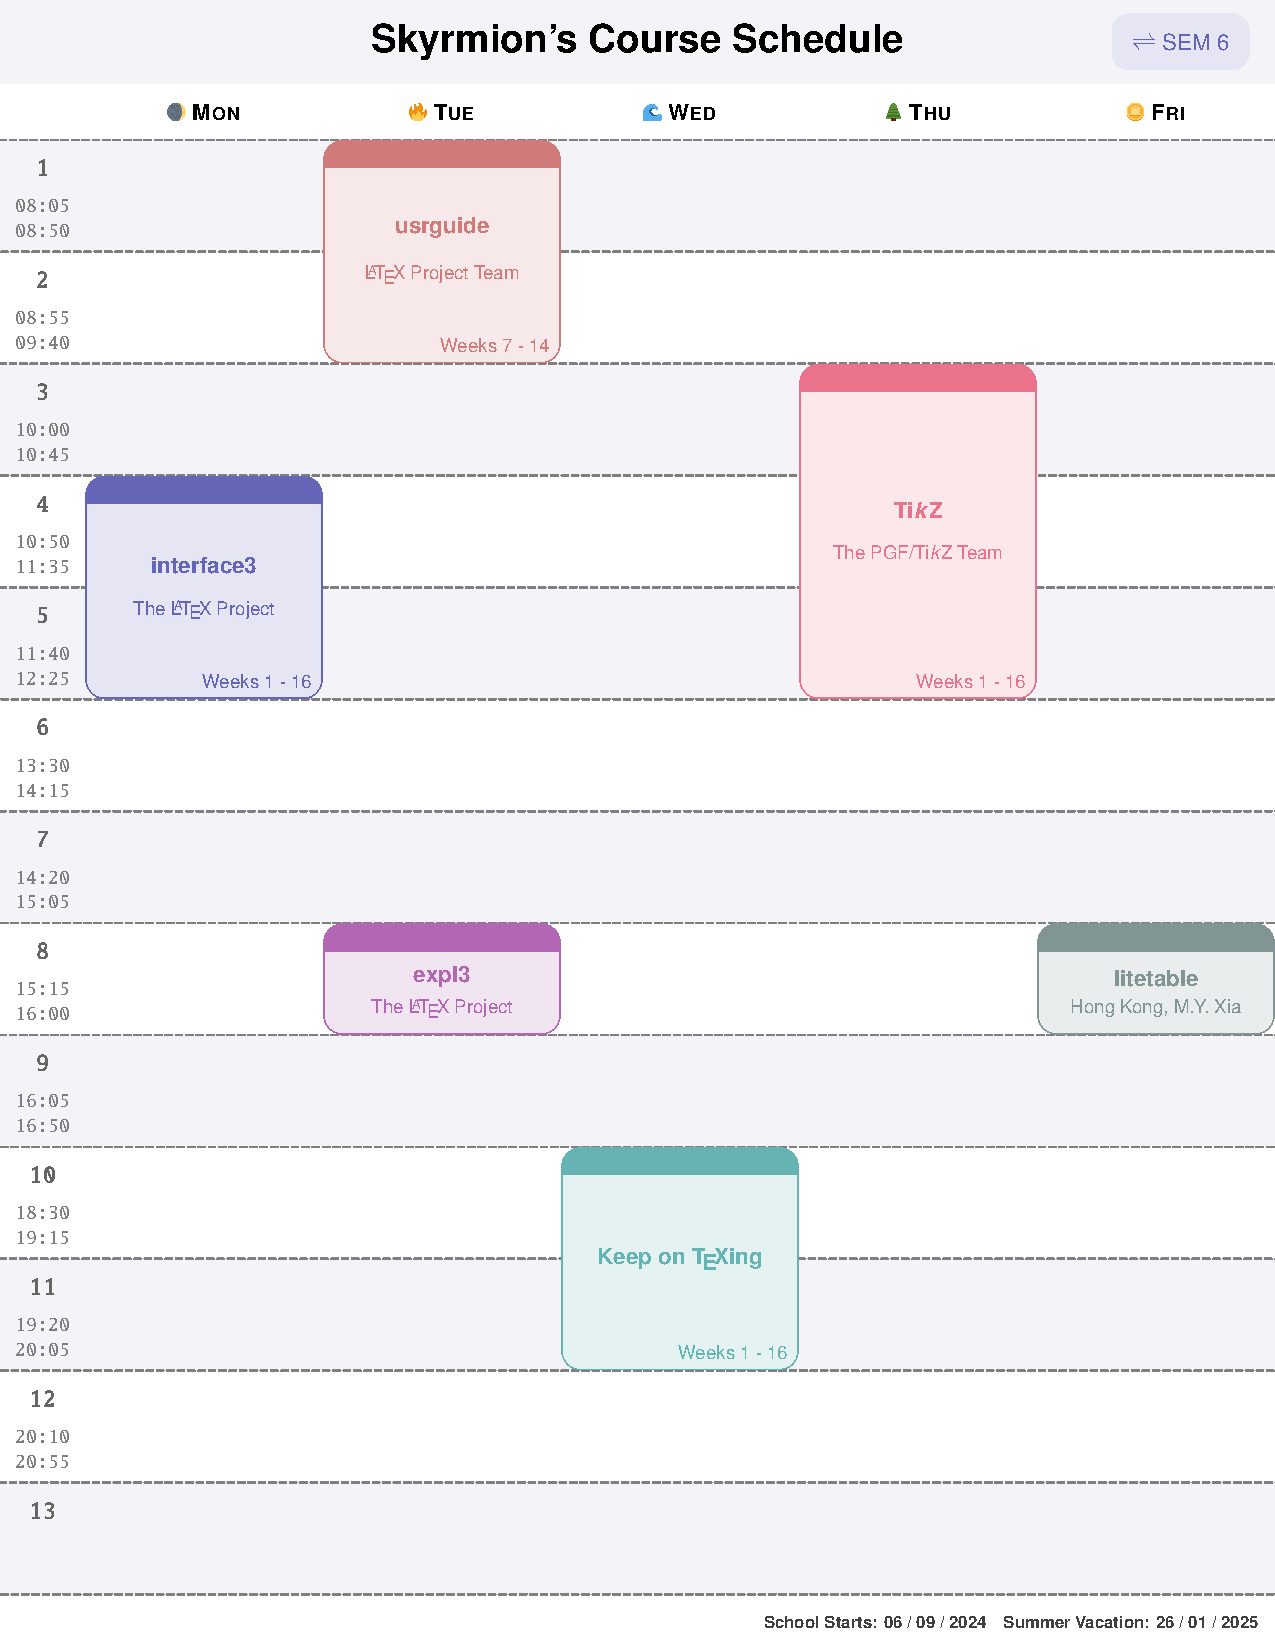
\includepdf[pages = 1]{litetable-demo.pdf}

\end{document}

% End of file litetable-en-us.tex
